\chapter{Emission Diagnostics}
\label{ch:emission}
\hl{This chapter will discuss emission measure (EM), differential EM (DEM), line intensities etc.
and how they are interpreted in observational and modeling contexts
Discuss how this is how we know anything about plasma in the solar atmosphere
Can discuss forward modeling as well; this sets us up for the rest of the thesis}
%
\par In solar physics (and astrophysics in general), all observational data must be collected through \textit{remote sensing} techniques rather than \textit{in situ} measurements due to the great distances and extreme environments inherent to the discipline. This means that atomic data and spectroscopy must be used to infer properties about the coronal plasma, including the temperature and density. To a good approximation, the hot, tenuous coronal plasma is \textit{optically thin} to radiation emitted in the visible, ultraviolet (UV), and x-ray bands. This means that, between the observer and where the radiation was produced, the photons were not scattered or absorbed and reemitted. As a result, the observed radiation contains signatures of the plasma that produced it and has not been polluted by some intermediate process.
%
\section{Spectral Line Intensity}
\label{sec:spectral_lines}
%
As discussed in \S\ref{sec:coronal_heating}, spectroscopy has been a critically important tool in solar physics since the discovery of the million-degree corona. Modern observing instruments and techniques have allowed for the collection of an unprecedented amount of data at increasingly higher spatial resolution and temporal cadence. However, interpreting this spectroscopic data in terms of useful plasma parameters (e.g. density and temperature) continues to pose a challenge to both observers and modelers alike.
%
\par The dominant emission mechanism in the high-temperature, low-density solar corona is \textit{bound-bound} emission,
\begin{equation}
	\label{eq:bound_bound}
	X_j^{+m}\to X_i^{+m} + h\nu_{j,i},
\end{equation}
where $X$ represents the atomic species, $m$ is the charge state, $h$ is Planck's constant, and $\nu_{j,i}$ is the frequency of the emitted photon of energy $\Delta E_{j,i} = h\nu_{j,i}=hc/\lambda_{j,i}$, with $j$ and $i$ representing the bound and lower energy states, respectively \citep{mason_spectroscopic_1994}. In this process, ion $X^{+m}$ spontaneously decays from excited state $j$ to lower-energy state $i$, emitting a photon of frequency $\Delta E_{j,i}$. The associated emissivity (power per unit volume) for the transition can then be written as 
\begin{equation}
	\label{eq:emissivity}
	P(\lambda_{j,i})=N_j(X^{+m})A_{j,i}\Delta E_{j,i},
\end{equation}
where $N_j(X^{+m})$ is the number density of element $X$ with charge state $+m$ in excited state $j$ and $A_{j,i}$ is the Einstein spontaneous emission coefficient. Thus, the power for a given spectral line is dependent on both the number of ions of a particular charge state and the number of ions in that particular charge state who are also in an excited state \citep{mason_spectroscopic_1994,bradshaw_collisional_2013}. Finally, this volumetric power can be related to the observed line intensity as at Earth,
\begin{equation}
	\label{eq:intensity}
	I(\lambda_{j,i}) = \frac{1}{4\pi R^2}\int_V \mathrm{d}V~P(\lambda_{j,i}),
\end{equation}
where the integral is taken over the entire sphere of radius $R$, where $R$ is the distance to the observer, and then normalized by the surface area of the sphere.
%
\par The next question is of course how these measured line intensities can be related to the properties of the coronal plasma. In Eq. \ref{eq:emissivity}, $A_{j,i}$ can be calculated from laboratory experiments for a given transition and $\Delta E_{j,i}$ is easily found provided $\lambda_{j,i}$ is known. The remaining quantity, $N_j(X^{+m})$ can be expressed as a series of ratios,
\begin{equation}
	\label{eq:density_jm}
	N_j(X^{+m})=\frac{N_j(X^{+m})}{N(X^{+m})}\frac{N(X^{+m})}{N(X)}\frac{N(X)}{N(H)}\frac{N(H)}{N_e}N_e,
\end{equation}
where $N(X^{+m})$ is the number density of element $X$ in charge state $+m$, $N(X)$ is the number density of element $X$, $N(H)$ is the number density of hydrogen, and $N_e$ is the electron number density \citep{mason_spectroscopic_1994}. Note that $N_j(X^{+m})$ has just been repeatedly multiplied by one in order to reexpress it in terms of the following ratios (from left to right in Eq. \ref{eq:density_jm}): fraction of $+m$-ions in excited state $j$, fraction of $X$ atoms in charge state $+m$, relative abundance of $X$ compared to hydrogen, and relative abundance of hydrogen compared to the number of electrons. The expression can be further simplified through the definition of the relative abundance $\mathrm{Ab}_X=N(X)/N(H)$ and the common approximation $N(H)/N_e\approx0.83$.
%
\par Eq. \ref{eq:emissivity}, and thus Eq. \ref{eq:intensity}, can be further simplified by invoking the \textit{coronal model} approximation. In optically-thin plasmas, it can be assumed that the collisional excitation and radiative decay occur from and to the ground state, respectively; in other words $i\to g$, with g representing the ground state. Additionally, the processes which determine the excitation level and those that determine the charge state are assumed to operate on disparate enough timescales such that the changes in energy level populations of the emitting ions, occurring on short timescales, can be decoupled from the changes in the charge state, occurring on longer timescales \citep{bradshaw_collisional_2013}. Using these assumptions, statistical equilibrium between the spontaneous decay and collisional excitation processes demands
\begin{equation}
	\label{eq:stat_eq}
	N_g(X^{+m})N_eC^e_{g,j} = N_j(X^{+m})A_{j,g},
\end{equation}
where $C^e_{g,j}$ is the electron collisional excitation rate between $g$ and $j$ \citep{bradshaw_collisional_2013}. Plugging Eqs. \ref{eq:stat_eq} and \ref{eq:density_jm} into Eq. \ref{eq:emissivity} and letting $N_g(X^{+m})\approx N(X^{+m})$ yields
\begin{equation}
	\label{eq:emissivity_simple}
	P(\lambda_{j,g})=(0.83)\mathrm{Ab}_X\Delta E_{j,g}\frac{N(X^{+m})}{N(X)}C^e_{j,g}N_e^2.
\end{equation}
Defining the \textit{contribution function} $G(T,\lambda_{j,g})=N(X^{+m})/N(X)C^e_{j,g}$, the intensity integral can be rewritten as
\begin{equation}
	I(\lambda_{j,g}) = \frac{(0.83)\mathrm{Ab}_X\Delta E_{j,g}}{4\pi R^2}\int_V\mathrm{d}V~N_e^2G(T,\lambda_{j,g}).
\end{equation}
If the plasma is isothermal over the emitting volume $V$, $G(T,\lambda_{j,g})$ comes outside the integral such that 
\begin{equation}
	\label{eq:intensity_isothermal}
	I(\lambda_{j,g}) = \frac{(0.83)\mathrm{Ab}_X\Delta E_{j,g}}{4\pi R^2}G(T,\lambda_{j,g})\langle\mathrm{EM}\rangle,
\end{equation}
where $\langle\mathrm{EM}\rangle=\int_V\mathrm{d}V~N_e^2$ is the average \textit{emission measure}. However, in many cases, this isothermal approximation does not hold such that the intensity integral must be expressed as 
\begin{equation}
	\label{eq:dem_integral}
	I(\lambda_{j,g}) = \frac{(0.83)\mathrm{Ab}_X\Delta E_{j,g}}{4\pi R^2}\int_V\mathrm{d}T~\phi(T)G(T,\lambda_{j,g}),
\end{equation}
where $\phi(T)=N_e^2\mathrm{d}V/\mathrm{d}T$ is the \textit{differential emission measure} ($\mathrm{DEM}$). 
%%
\section{Differential Emission Measure}
\label{sec:dem}
%
\par The $\mathrm{DEM}$ and $\mathrm{EM}$ provide information about the temperature distribution of the plasma. In particular, the $\mathrm{DEM}$ is a measure of the amount of emitting material at a particular temperature $T$ in the plasma. Thus, the $\mathrm{DEM}$ is an observable that any viable theory of coronal heating should be able to predict with reasonable accuracy \citep{golub_solar_2010}. Furthermore, because the $\mathrm{DEM}$ is a one-dimensional function, it provides a simple and powerful characterization of the multi-thermal coronal plasma. Unfortunately, calculating these quantities from observed line intensities is difficult because of both mathematical and data availability issues. Looking back to Eq. \ref{eq:intensity_isothermal}, one can see that, provided the line intensities and contribution functions are available over a significant range of temperatures, the emission measure can be calculated algebraically.
%
\subsection{Reconstruction Techniques}
\label{subsec:reconstruction}
%
\par If the plasma is assumed to be approximately isothermal over the emitting volume, say at temperature $T_C$, the contribution function can be taken outside of the integral as in Eq. \ref{eq:intensity_isothermal}. Furthermore, if the plasma is assumed to have a constant density over the emitting volume as well, then $\langle\mathrm{EM}\rangle\approx N_e^2V$. To determine the $T_C$, the temperature of the plasma, the emission measure for each spectral line is calculated over the appropriate temperature range,
\begin{equation}
	\label{eq:em_loci}
	\langle\mathrm{EM}(T)\rangle=4\pi R^2\frac{I_j}{(0.83)\mathrm{Ab}_X\Delta E_jG_j(T,N_e)},
\end{equation}
where the contribution function $G$ for a particular spectral line $j$ at temperature $T$ and density $N_e$ can be calculated using the CHIANTI atomic database \citep{dere_chianti_1997,landi_chiantiatomic_2013}. Typically, this procedure is done for a sufficiently large sample of observed spectral line intensities and the corresponding $\langle\mathrm{EM}(T)\rangle$ curves plotted on top of each other. Because of the isothermal assumption, these curves should intersect at a common point, $(T_C,\langle\mathrm{EM}(T_C)\rangle)$ \citep{landi_chianti-atomic_2002}. Of course this isothermal condition is never actually met; thus, all curves tend to meet in a region of intersection. The more multithermal the plasma is, the broader the region of intersection will be and, consequentially, the value of $T_C$ will be less constrained, leading to indeterminate measurements of the plasma temperature. An example for a simulated data set with a very narrow temperature distribution and thus a well-determined value of $T_C$ is shown in Fig. \ref{fig:em_loci_example}. 
%
\begin{figure}[ht]
	\centering
	\subfigure[]{%
	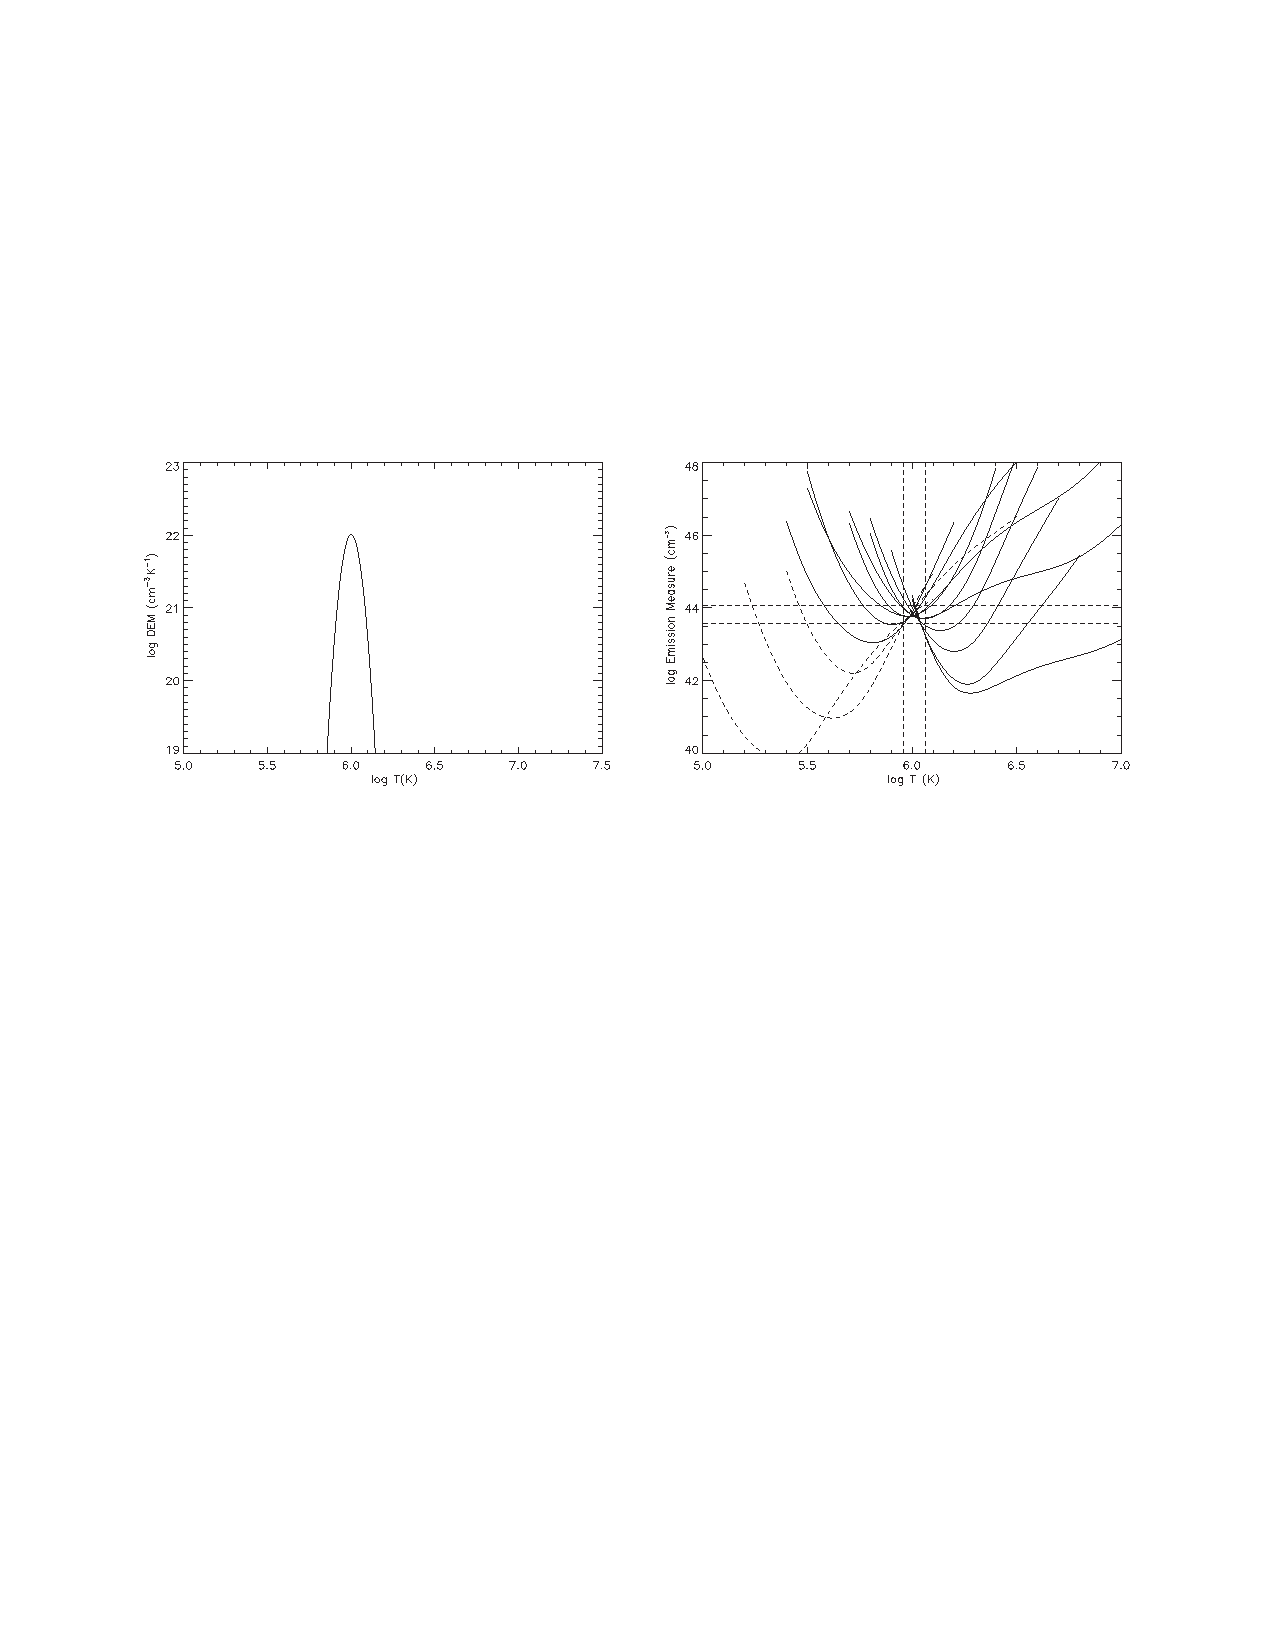
\includegraphics[width=0.8\textwidth]{figures/em_loci.pdf}
	\label{fig:em_loci_example}}
	\subfigure[]{%
	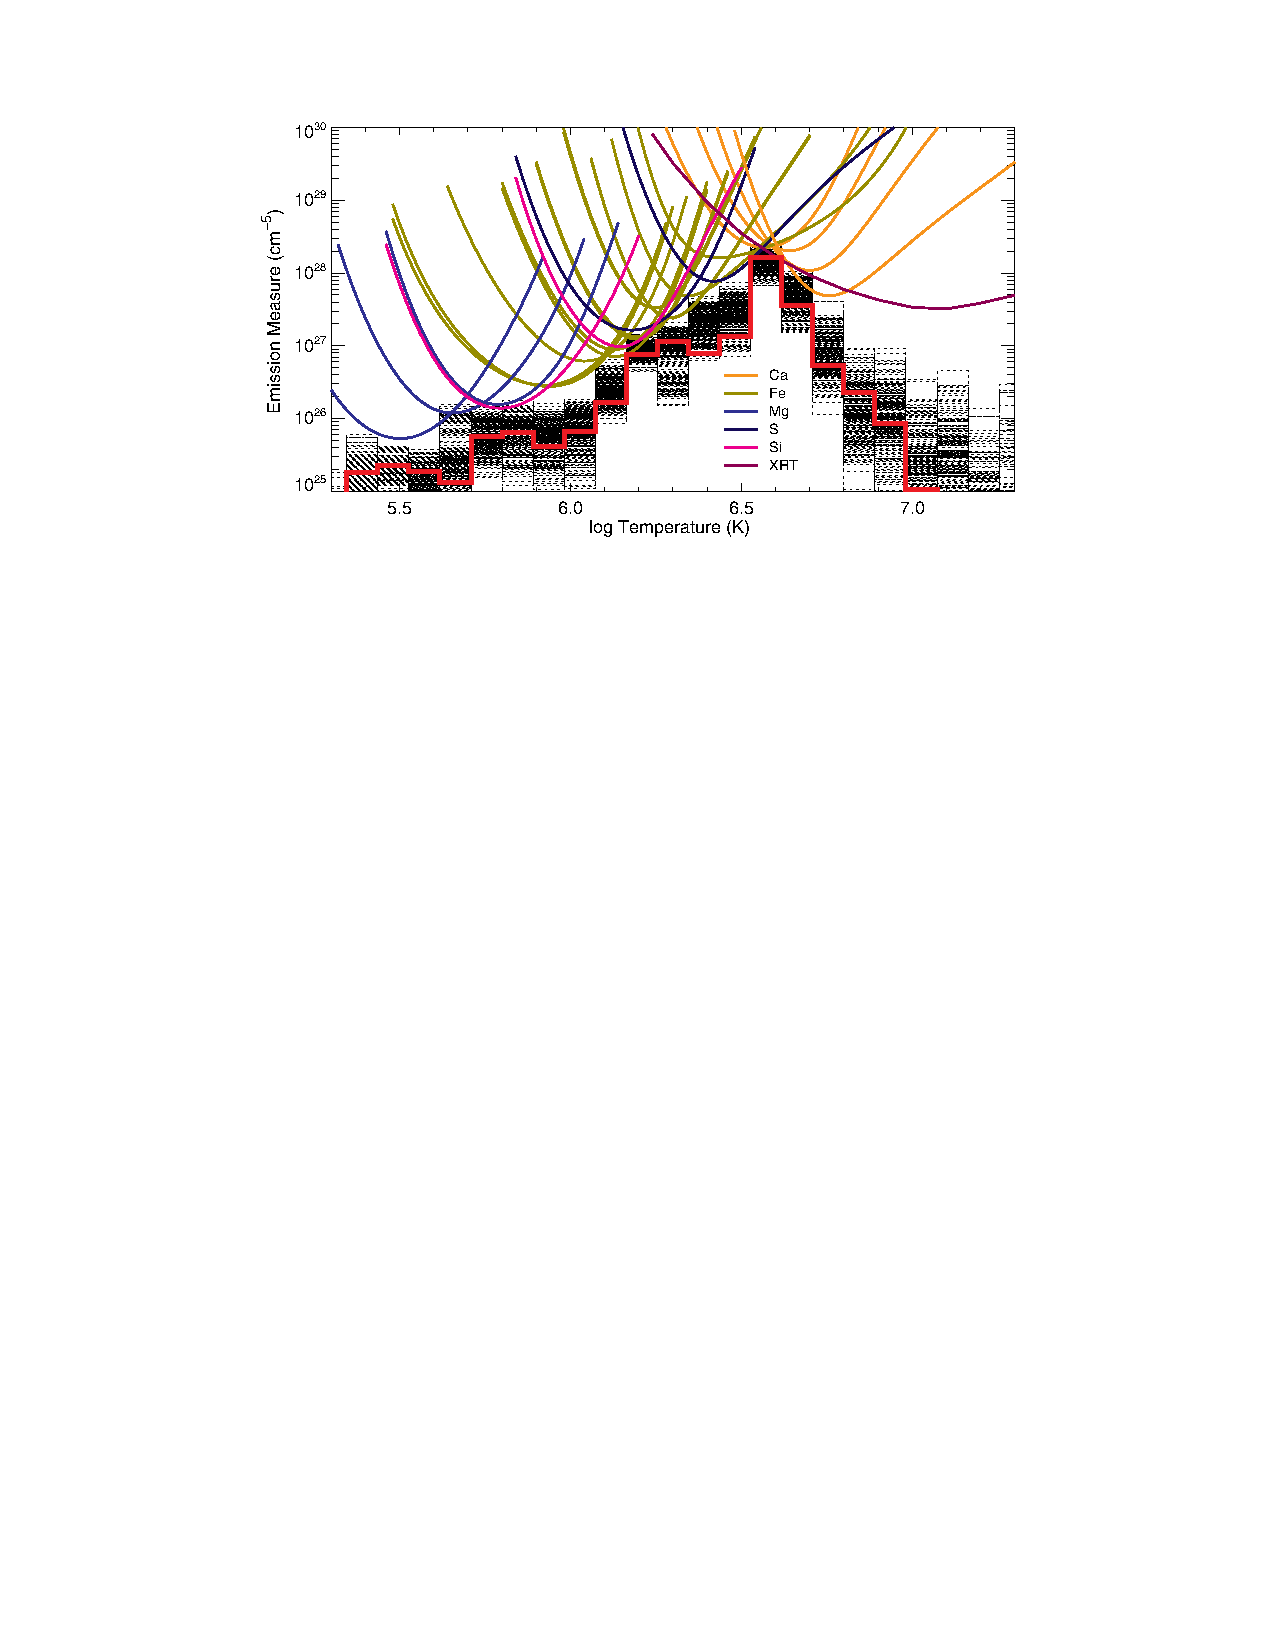
\includegraphics[width=0.75\textwidth]{figures/dem_em_loci.pdf}
	\label{fig:dem_example}}
	\caption{\textbf{(a)} Simulated $\mathrm{DEM}$ curve and the resulting $\mathrm{EM}$ loci reconstruction. From the $\mathrm{DEM}$ curve, the plasma is approximately isothermal, being sharply peaked about 1 MK. Correspondingly, the $\mathrm{EM}$ loci curves intersect in a region centered on 1 MK, allowing for a well-constrained determination of $T_C$. Image taken from \citet{landi_isothermality_2010}. \textbf{(b)} Emission measure distribution reconstruction for an active region core. The colored curves show the emission measure calculation using the $\mathrm{EM}$ loci method. The black and red histograms show the $\mathrm{DEM}(T)\mathrm{d}T$ reconstructed using the MCMC method of \citet{kashyap_markov-chain_1998}. Here, the $\mathrm{DEM}$ is multiplied by the temperature bin for comparison with the $\mathrm{EM}$ loci calculation. Image taken from \citet{warren_constraints_2011}}
	\label{fig:dem_em_loci_example}
\end{figure}
%
\par Relaxing the isothermal assumption introduces a great deal more complexity. Unlike $\langle\mathrm{EM}\rangle$, $\phi(T)$ cannot be determined algebraically; instead, Eq. \ref{eq:dem_integral}, a Fredholm equation of the first kind, must be inverted to find $\phi(T)$, a task that poses well-known mathematical difficulties \citep{kashyap_markov-chain_1998}. One method for performing such an inversion is a discretization of Eq. \ref{eq:dem_integral}
\begin{equation}
	\label{eq:disc_dem_integral}
	I_j = \frac{(0.83)\mathrm{Ab}_X\Delta E_j}{4\pi R^2}\sum_{k=1}^N\phi_k\int^{T_{k+1}}_{T_k}\mathrm{d}T~G_j(T),
\end{equation}
where $j$ labels the spectral line and $[T_{k+1},T_k]$ is the temperature interval over which $\phi_k$ is constant. For each measured line intensity $I_j$, $\phi_k$ for $1\le k\le N$ are determined through some minimization procedure \citep{landi_monte_2012}. To calculate the $\mathrm{DEM}$ curve, an arbitrary spline or polynomial is first assumed; subsequent corrections at $T_{eff,j}$, the temperature of maximum abundance for the line intensity $I_j$, are then calculated and a spline interpolation applied to these corrections for the entire temperature range $[T_1,T_N]$. This correction is then applied to initial curve and the corrected curve is used as the initial $\mathrm{DEM}$ on the next iteration \citep{landi_monte_2012}. This method of course has the disadvantage that a functional form for the $\mathrm{DEM}$ must be chosen \textit{a priori}, biasing the temperature distribution. Additionally, a poor choice of temperature interval in Eq. \ref{eq:disc_dem_integral} can oversmooth the $\mathrm{DEM}$ curve or cause convergence issues.
%
\par An alternative method for calculating the $\mathrm{DEM}$ that has begun to gain popularity is the Markov-chain Monte Carlo (MCMC) method developed by \citet{kashyap_markov-chain_1998}. Using a Bayesian approach, the goal of this method is to maximize the probability $P(X,F)$ of obtaining observed line intensities $F=(F_1,F_2,\ldots,F_n)$ from a $\mathrm{DEM}$ characterized by a set of parameters $X=(X_1,X_2,\ldots,X_m)$. First, a set of $N$ temperature bins is chosen such that within each bin, the plasma is assumed to be isothermal and can be described by an emission measure $\mathrm{EM}_i$. As a result, the set of parameters $X$ that describe the $\mathrm{DEM}$ is $X=(\mathrm{EM}_1,\mathrm{EM}_2,\ldots,\mathrm{EM}_N)$. To maximize $P(X,F)$, the parameters of $X$ are varied step by step such that the change introduced only depends on the parameters of the previous step. This new set of parameters $X^{\prime}$ has a new probability $P(X^{\prime},F)$ and this new set of parameters is accepted or rejected based on the Metropolis algorithm \citep{metropolis_equation_1953}. The emission measure values in each bin thus comprise the $\mathrm{DEM}$. Unlike other reconstruction methods, the MCMC method has the benefit of not assuming \textit{a priori} a functional form for the $\mathrm{DEM}$ curve and does not impose unphysical smoothness constraints on the final solution \citep{landi_monte_2012}.
%
\subsection{Scaling Laws}
\label{subsec:scaling}
%
%\hl{Here something about emission measure scaling with temperature + observational results supporting + simulation results supporting + introduce hot emission}
\par From these emission measure distributions, simple observables can be calculated that any viable heating model should be able to produce. The most popular of these observables is the well-known scaling between the emission measure and the temperature, 
\begin{equation}
	\mathrm{EM}\propto T^a.
\end{equation}
This scaling, first proposed by \citet{jordan_energy_1980}, has since been validated by both simulation and observation. A summary of model and observational results for the $a$ parameter can be found in Table \ref{tab:em_scalings}. Looking at the sample emission measure distributions in Fig. \ref{fig:dem_em_loci_example}, it can be seen that, for isothermal (Fig. \ref{fig:em_loci_example}) and multithermal (Fig. \ref{fig:dem_example}) plasmas, the emission measure distribution tends to be strongly peaked. When determining the scaling parameter $a$, it is common perform a linear fit in $(\log{T},\log{\mathrm{EM}})$ coolward of the peak, typically between 6.0 and $\log{T_{peak}}$, where $T_{peak}$ is the temperature at which $\mathrm{EM}_{max}$ occurs. Observations of the inter-moss regions of active region cores, where the emission is less likely to be contaminated by transition region lines, indicate that $2\lesssim a\lesssim5$. Table \ref{tab:em_scalings} summarizes these findings. This large range of values is most likely due to both uncertainties in the atomic data as well as the variety of techniques used to reconstruct the emission measure distribution (see \S\ref{subsec:reconstruction}).
%
\par These scalings have also recently been studied in the context of simulation. \citet{mulu-moore_can_2011}, using a 1D hydrodynamic model, constructed emission measure distributions for a $3\times3$ parameter space of loop length and equilibrium temperature using a single impulsive heating function. They found that this ``long nanoflare storm'' heating scenario, in which impulsive heating events occur infrequently on sub-resolution strands, produced emission measure slopes that were too small to adequately account for observations. Using an advanced forward modeling technique and a different 1D hydrodynamic model, \citet{bradshaw_diagnosing_2012} and \citet{reep_diagnosing_2013} investigated the effect of low-frequency and high-frequency nanoflare heating, respectively, on the resulting emission measure. \citet{bradshaw_diagnosing_2012} found that low-frequency heating could not account for the entire range of observed emission measure slopes while \citet{reep_diagnosing_2013} showed high-frequency heating could. Additionally, \citet{cargill_active_2014}, using an efficient ``0D'' hydrodynamic simulation (see \S\ref{sec:ebtel}), showed that $a$ can vary from 2 to greater than 5 depending on the heating frequency, whether the heating spectrum follows a power-law, and how the heating scales with the time between successive heating events.
%
\begin{table}[ht]
	\centering
	\caption{Summary of emission measure scalings from observational and modeling studies. Scalings are typically calculated coolward of the emission measure peak and typically range from 2 to 5. Adapted from \citet{bradshaw_diagnosing_2012}.\label{tab:em_scalings}}
	\begin{tabular}{L{4cm} l l l}
		\hline\hline
		Slopes, $a$ & Range of $\log{T}$ & Type & Reference \\
		\hline
		3.26 & 6.00-6.60 & observation & \citet{warren_constraints_2011} \\
		2.17 &  & model & \\
		\hline
		3.20 & 6.00-6.50 & observation & \citet{winebarger_using_2011} \\
		\hline
		2.08-2.47 \\ (background) & 5.50-6.55 & observation & \citet{tripathi_emission_2011} \\
		2.05-2.70 \\ (background subtracted) &  &  & \\
		\hline
		1.60-2.00 \\ (photospheric abundances) & 6.00-[6.60-6.80] & model & \citet{mulu-moore_can_2011} \\
		2.00-2.30 \\ (coronal abundances) &  &  & \\
		\hline
		1.70-4.50 & 6.00-6.60 & observation & \citet{warren_systematic_2012} \\ 
		\hline
		1.91-5.17 & 6.00-[6.30,6.80] & observation & \citet{schmelz_cold_2012} \\
		\hline
		0.58-2.24 \\ (low-frequency nanoflares) & 6.00-$\log{T_{peak}}$ & model & \citet{bradshaw_diagnosing_2012} \\
		\hline
		0.79-3.65 \\ (nanoflare trains) & 6.00-$\log{T_{peak}}$ & model & \citet{reep_diagnosing_2013} \\
		\hline
		$\sim2-\sim7$ \\ (low- to high-frequency heating) & [6.00-6.25]-$\log{T_{peak}}$ & model & \citet{cargill_active_2014} \\
		\hline
	\end{tabular}
\end{table}
%
\par \hl{paragraph about scaling hotward of the peak and why this is important for nanoflare heating; briefly talk about model emission measure versus forward modeling or observed emission measure to lead into forward modeling section}
%
%%
\section{Forward Modeling}
\label{sec:charge_state}
%
\par \hl{Talk about forward modeling procedure, why it is important, how it is done, CHIANTI, hydrodynamics, some nice pictures}
%
%%